%//////////////////////////////////
%/// P R E A M B L E

\documentclass[a4paper, 12pt]{article}

\usepackage[utf8]{inputenc}
\usepackage[singlespacing]{setspace}
\usepackage{amsmath}
\usepackage{mathtools}
\usepackage{caption}
\usepackage{float}
\usepackage{graphicx}
\usepackage{multicol}
\usepackage{gensymb}
\usepackage{breqn}
\usepackage{indentfirst}
\usepackage{siunitx}
\usepackage{tabularx, booktabs}
\newcolumntype{Y}{>{\centering\arraybackslash}X}

\usepackage{pdfpages}

\usepackage{multicol}
\usepackage{supertabular}

\usepackage{svg}

\widowpenalty = 4500
\clubpenalty  = 4500

\setlength{\jot}{10pt} %indents


\newcommand*\dif{\mathop{}\!\mathrm{d}}

%%========================================
%% circuitikz properties
\usepackage[european, straightvoltages]{circuitikz}
%\ctikzvalof{voltage/distance from node = .2}
%\ctikzset{voltage/distance from node  =.5}% in \pgf@circ@Rlen units
%\ctikzset{voltage/distance from line  =.25}% pos. between 0 and 1
%\ctikzset{voltage/bump b/.initial     =1.5}%

\ctikzset{current/distance            = .618}


%%========================================

%%
%% Path settings
%%
\graphicspath{ {./graphics/} }


%//////////////////////////////////
%/// D O C U M E N T
\begin{document}

%%%%%%%%%%%%%%%%%%%%%%%%%%%%%%%%%%%%%
  \includepdf{Deckblatt.pdf}
  
\includepdf{./titlepage/titlepage.pdf}
%%%%%%%%%%%%%%%%%%%%%%%%%%%%%%%%%%%%%

\section{Vorbereitungsaufgaben}
%1.1
\subsection{}

  \begin{center}
    \begin{align*}
      i(t) = \hat{I} \cdot \cos(\omega t + \phi_i)
    \end{align*}
  \end{center}

  \vspace{0.013155617496424828\columnwidth}


    %Resistor
  (3)\\
  \begin{center}
    \begin{circuitikz}[european voltages, european resistors]
      \draw (0,0) to[R, l=$R$, i=$i(t)$, v=$u_R(t)$, color = black] (2,0);
    \end{circuitikz}

    \begin{align*}
      u_R(t)  & = R \cdot i(t)\\
              & = \underbrace{R \cdot \hat{I}}_{ \mathclap{\hat{U}_R }} \cdot \cos(\omega t + \phi_i)\\
      \intertext{Da sich die Phase nicht ändert, gilt außerdem $\phi_i = \phi_u$ und somit:}
      \Aboxed{u_R(t)  & = \hat{U} \cdot \cos(\omega t + \phi_u)}\\
    \end{align*}

  \end{center}

  (4)\\
  \begin{center}
    %inductance
    \begin{circuitikz}[european voltages, european inductors]
      \draw (0,0) to[L, l=$L$, i=$i(t)$, v=$u_L(t)$, color = black] (2,0);
    \end{circuitikz}

    \begin{align*}
      u_L(t)  & = L \cdot \frac{\dif i(t)}{\dif t}\\
              & = L  \cdot \hat{I} \cdot \frac{\dif}{\dif t}\left( \cos(\omega t + \phi_i)\right)\\
              & = -\underbrace{ \omega \cdot L \cdot \hat{I} }_{ \mathclap{\hat{U}_L} } \cdot \sin(\omega t + \phi_i)\\
      \intertext{Um die Spannung ($-\sin{x}$) wieder durch $\cos{x}$ auszudrücken, muss auf den ursprünglichen Phasenwinkel $\pi / 2$ addiert werden:}
      \Aboxed{ u_L(t)  & = \hat{U}_L \cdot \cos(\omega t + \underbrace{\phi_i + \frac{\pi}{2}}_{ \mathclap{\phi_u}})}\\
    \end{align*}

  \end{center}

  (5)\\
  \begin{center}
    %capacitance
    \begin{circuitikz}[european voltages, european resistors]
      \draw (0,0) to[C, l=$C$, i=$i(t)$, v=$u_C(t)$, color = black] (2,0);
    \end{circuitikz}

    \begin{align*}
      u_C(t) & = \frac{\hat{I}}{C} \cdot \int_0^t{i(t) \dif t}\\
             & = \frac{\hat{I}}{C} \cdot \int_0^t{ \cos{(\omega t + \phi_i)} \dif t}\\
             & = \frac{\hat{I}}{C} \cdot \frac{1}{\omega} [\sin{(\omega t + \phi_i)}]_0^t + \underbrace{U_0}_{\mathclap{\text{initialer Ladezustand}}}\\
             & = \underbrace{\frac{\hat{I}}{C \cdot \omega}}_{\mathclap{\hat{U}_C}} [\sin{(\omega t + \phi_i)} - \sin{(\phi_i)}] + U_0\\
       \intertext{Um die Spannung ($\sin{x}$) wieder durch $\cos{x}$ auszudrücken, muss von dem ursprünglichen Phasenwinkel $\pi / 2$ subtrahiert werden:}
     \Aboxed{ u_C(t)  & = \hat{U}_C \cdot \left(\cos(\omega t + \underbrace{\phi_i - \frac{\pi}{2}}_{\mathclap{\phi_u}}) - \cos{(\underbrace{\phi_i - \frac{\pi}{2}}_{\mathclap{\phi_u}})}\right) + U_0}\\
    \end{align*}

  \end{center}

%1.2
\subsection{}
  (3)\\
  \begin{gather*}
    u_R(t)   = R \cdot i(t)\\
    i(t)      = \frac{u(t)}{R}\\
  \end{gather*}

  (4)\\
  \begin{gather*}
        u_L(t) = L \cdot \frac{\dif i(t)}{\dif t}\\
    \dif i(t)  = \frac{1}{L} \cdot u_L(t) \dif t\\
        i(t)   = \frac{1}{L} \cdot \int_0^t{u_L(t) \dif t} + i_0\\
  \end{gather*}
  \indent(5)\\
  \begin{gather*}
    u_C(t)   = \frac{1}{C} \cdot \int_0^t{i(t) \dif t}\\
    i(t)     = C \cdot \frac{\dif u_C(t)}{\dif t}\\
  \end{gather*}

%1.3
\subsection{}
  Zur Anwendung der symbolischen Methode werden folgende Bedingungen vorausgesetzt:
  \begin{itemize}
    \item \emph{Linearität}: Die Kenngrößen der Elemente $R, L, C$ sind von den Kenngrößen der Erregung ($U, I, \omega$) unabhängig
    \item Es liegt eine \emph{harmonische Erregung} ($\sin \text{/} \cos$) vor
    \item Der \emph{stationäre Zustand} ist erreicht, das System ist "eingeschwungen" und es treten keine Schaltvorgänge auf
  \end{itemize}

%1.4
\subsection{}
  Der \emph{Betragsgang} ist die Funktion $\text{f}(\omega)$, die den Verlauf des Verhältnisses der Amplituden (komplexer Betrag) oder Effektivwerte zweier Größen (z.B. Aus -und Eingangssignal) mit der (Kreis-)Frequenz abbildet.
  $$ \text{f}(\omega) = \frac{ \mid \underline{U}_2 \mid }{ \mid \underline{U}_1 \mid } =  \frac{ U_{2_eff} }{ U_{1_eff} }$$\\

  Der \emph{Phasengang} $\phi(\omega)$ ist das von der (Kreis-)Frequenz abhängige Argument des komplexen Verhältnisses des Aus- und Eingangssignals.
  $$\phi(\omega) = \text{arg} \left( \frac{ \underline{U}_2 }{ \underline{U}_1 } \right)$$\\

  %\vspace{0.021276873\paperheight}
  Sind Real- und Imaginärteil dieses komplexen Verhältnisses gleich, so wird das Amplitudenverhältnis $1/\sqrt{2}$ und die Phasenverschiebung $45 \degree$. Die dabei präsente Frequenz wird dann \emph{Grenzfrequenz} genannt.
  $$ \mid \text{Re}\left( \frac{ \underline{U}_2 }{ \underline{U}_1 } \right) \mid = \mid \text{Im}\left( \frac{ \underline{U}_2 }{ \underline{U}_1 } \right) \mid$$

%1.5
%\pagebreak
\subsection{}
  Im Folgenden wurden normierte Darstellungen der Betragsgänge gewählt, um von den Kenngrößen unabhängige Graphen zu erhalten. Zusätzlich sind die Abszissen dieser logarithmisch eingeteilt.

  \begin{center}
  \subsubsection*{Hochpassfilter (HP)}

    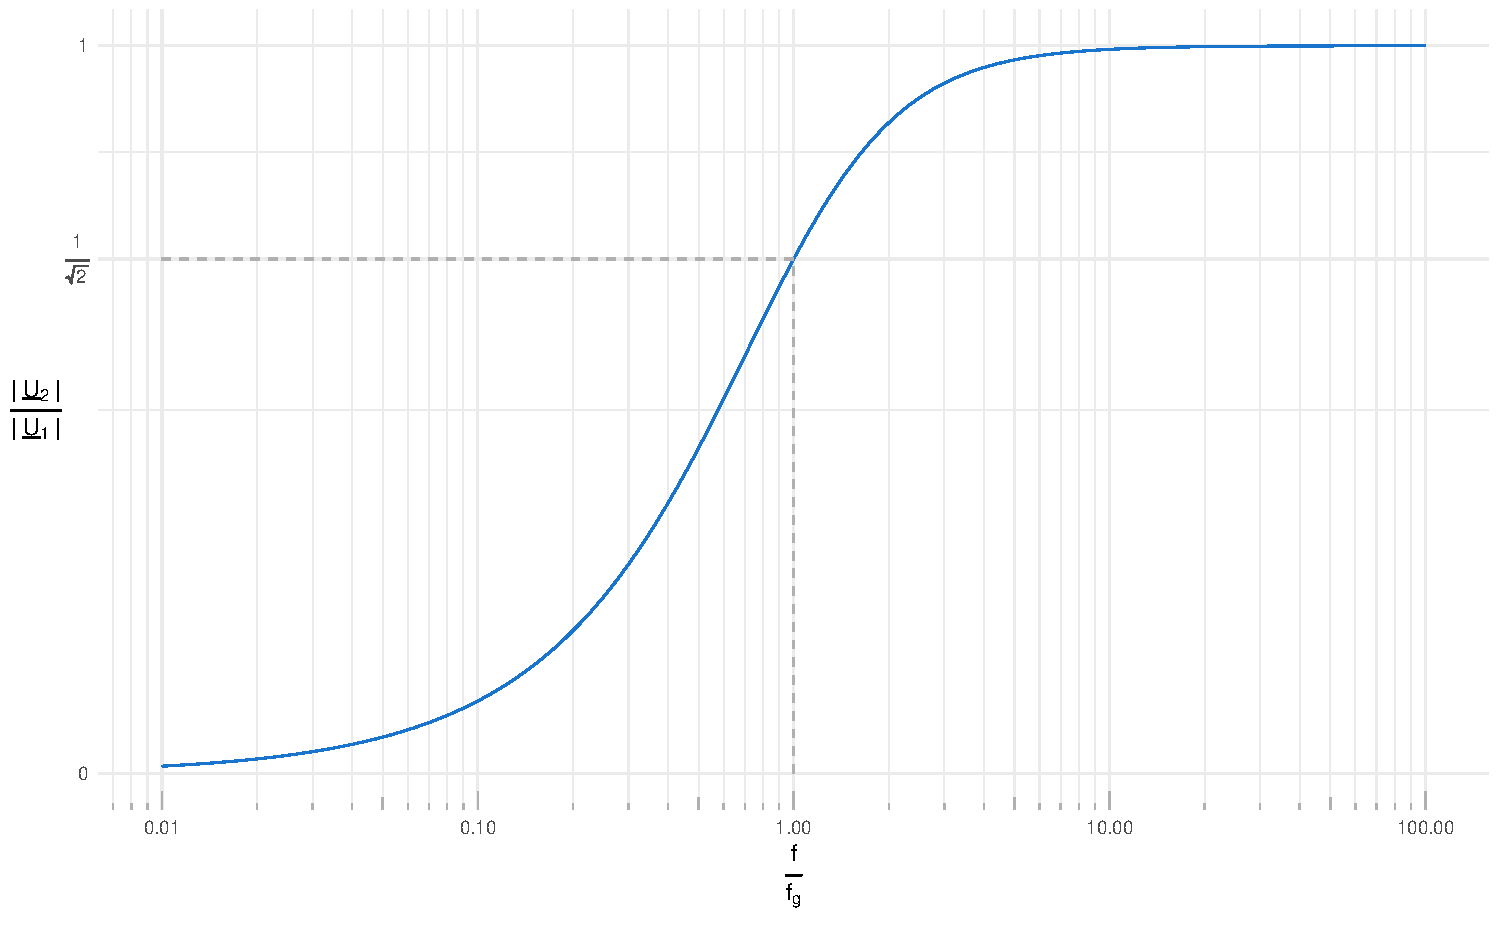
\includegraphics[scale=0.5]{./R/RL_HP/RL_HP_clean_alt.pdf}

  \vspace{0.021276873\paperheight}

  \subsubsection*{Tiefpassfilter (TP)}

    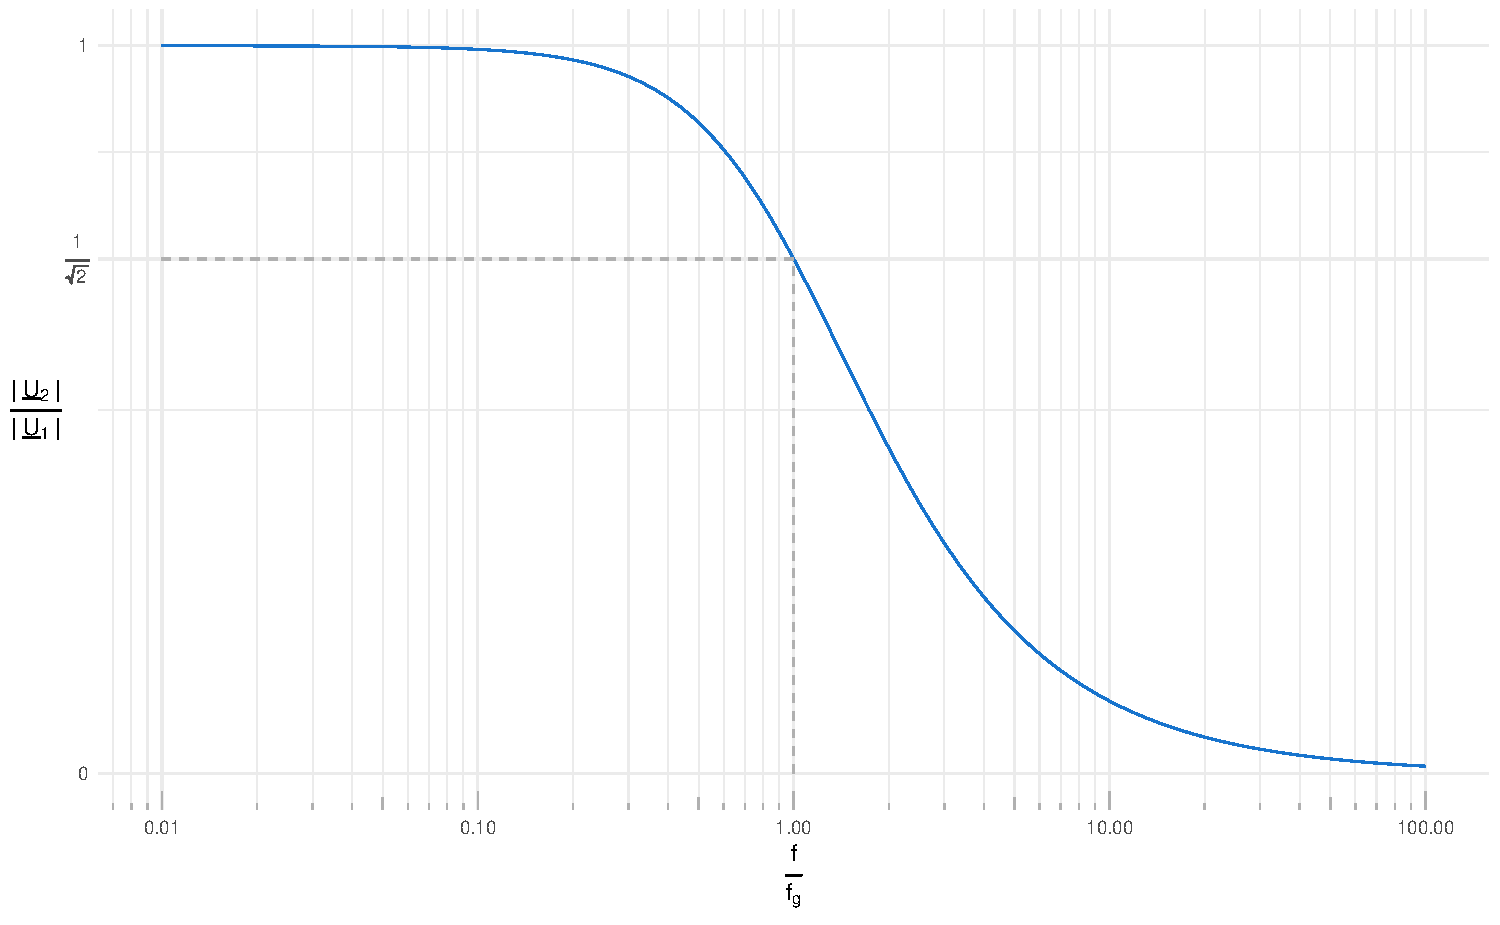
\includegraphics[scale=0.5]{./R/RC_LP/RC_LP_clean.pdf}

  \subsubsection*{Bandpass (BP)}

    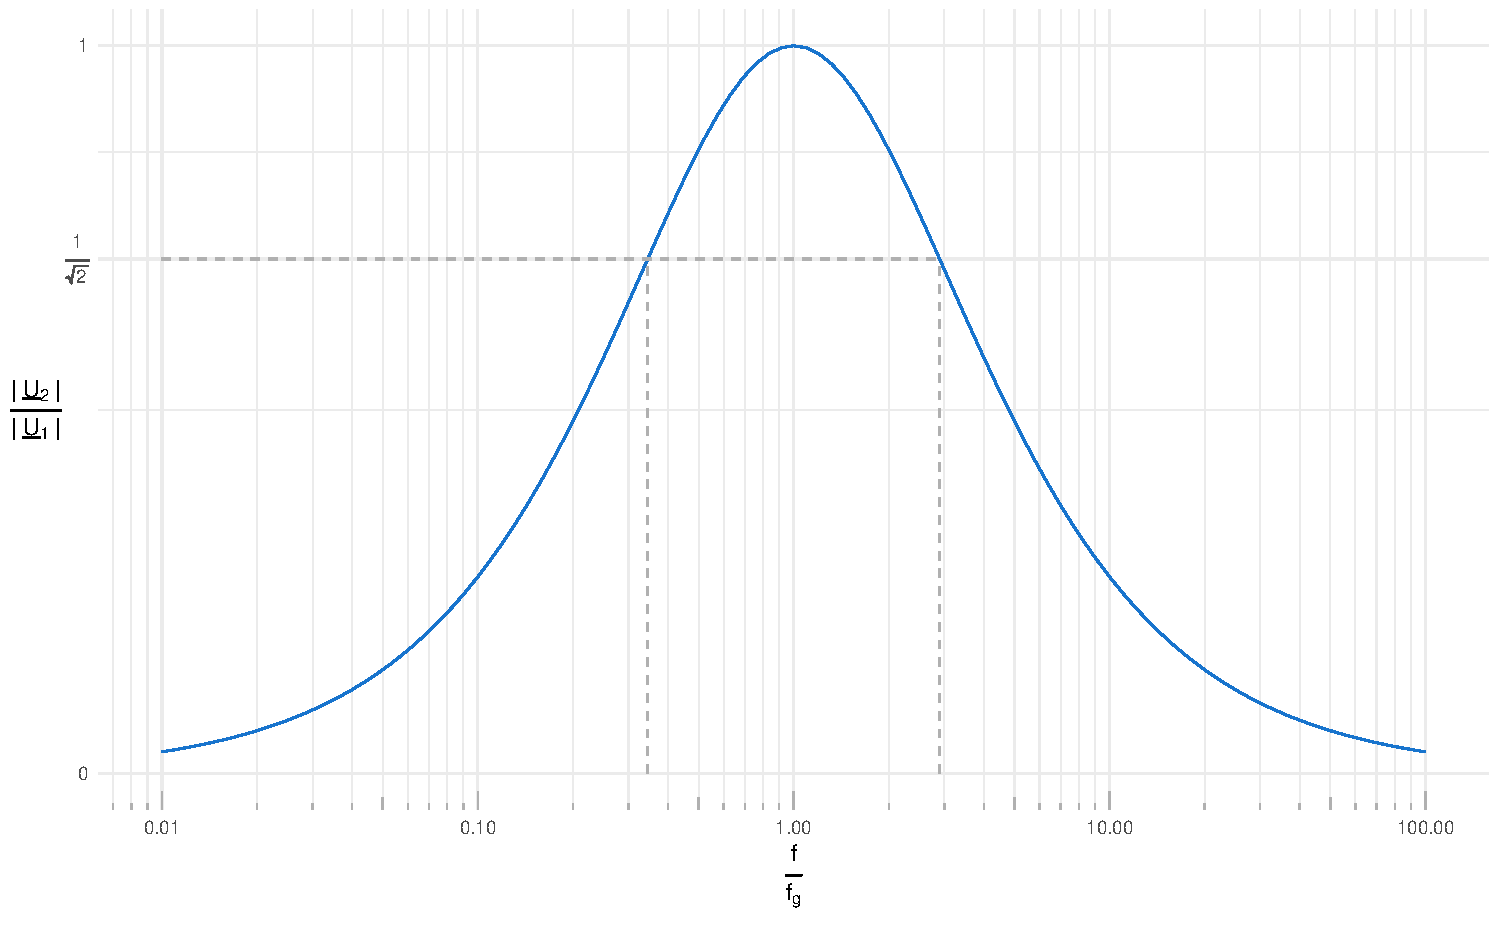
\includegraphics[scale=0.5]{./R/Band/BP/BP_clean.pdf}

  \vspace{0.021276873\paperheight}

  \subsubsection*{Bandsperre (BS)}

    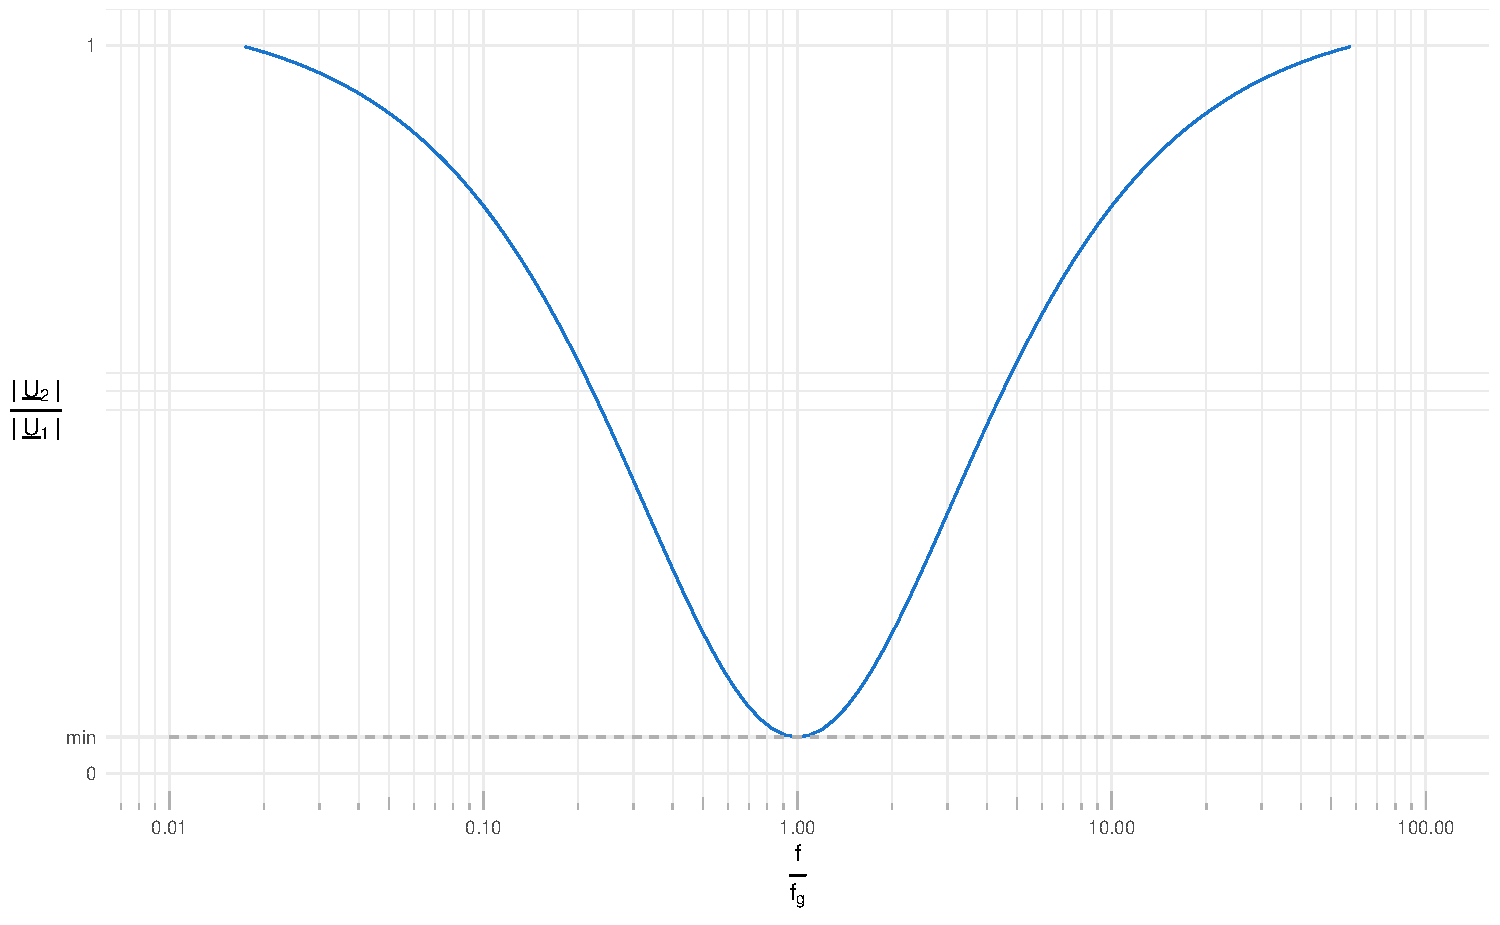
\includegraphics[scale=0.5]{./R/Band/BS/BS_clean.pdf}

  \end{center}

%1.6
\subsection{}

  \subsubsection*{RC-Tiefpass}

    \begin{center}
      \begin{circuitikz}

        \draw (0,0) to[open,v^=$U_1$, o-o] (0,-3);
        \draw (.05,0) to[R, l=$R$] (4,0); % kinda hacked
        \draw (4,0) to[open] (6,0);
        \draw (4,0) -- (6,0);
        \draw (4,0) to[C, l=$C$, *-*] (4,-3);
        \draw (6,0) to[open,v^=$U_2$,o-o] (6,-3);
        \draw (5.95,-3) to[short] (0.05,-3);

      \end{circuitikz}
    \end{center}

    \begin{gather*}
      \frac{\underline{U}_2}{\underline{U}_1} = \frac{\frac{1}{j \omega C}}{R +\frac{1}{j \omega C}} = \frac{1}{1 + j R \omega C}\\
    \end{gather*}

    Amplitude:
      \begin{gather*}
        \frac{\mid \underline{U}_2 \mid}{\mid \underline{U}_1 \mid} = \frac{\mid 1 \mid}{\mid 1 + j R \omega C\mid} = \frac{1}{\sqrt{1+\omega^2R^2C^2}}\\
      \end{gather*}

    Phase:
      \begin{gather*}
        \phi = \text{arg} \left( \frac{ \underline{U}_2 }{ \underline{U}_1 } \right) = 0 - \arctan{\frac{\omega R C}{1}} = -\arctan(\omega R C)\\
      \end{gather*}

    Grenzfrequenz:
      \begin{gather*}
        \mid \text{Re}\left( \frac{ \underline{U}_2 }{ \underline{U}_1 } \right) \mid = \mid \text{Im}\left( \frac{ \underline{U}_2 }{ \underline{U}_1 } \right) \mid\\
        \text{Nach komplex-konjugierter Erweiterung:}\\
        \frac{1}{1 + \omega_g^2 R^2 C^2} = \frac{\omega_g R C}{1 + \omega_g^2 R^2 C^2}\\
      \end{gather*}

      \begin{gather*}
        \omega_g R C = 1\\
        \omega_g = \frac{1}{R C}
      \end{gather*}

    Normierung:
        \begin{gather*}
          \frac{\mid \underline{U}_2 \mid}{\mid \underline{U}_1 \mid} \left( \frac{\omega}{\omega_g} \right) = \frac{1}{\sqrt{1+ \left( \dfrac{\omega}{\omega_g} \right)^2}} = \frac{1}{\sqrt{1+\left ( \dfrac{f}{f_g} \right)^2}}
        \end{gather*}

        \begin{gather*}
          \phi \left( \frac{\omega}{\omega_g} \right) = -\arctan{ \frac{\omega}{\omega_g} }
        \end{gather*} \\

      Betragsgang: \\ \indent \indent siehe 1.5: Tiefpassfilter\\\\
      \indent Phasengang:
        \begin{center}
          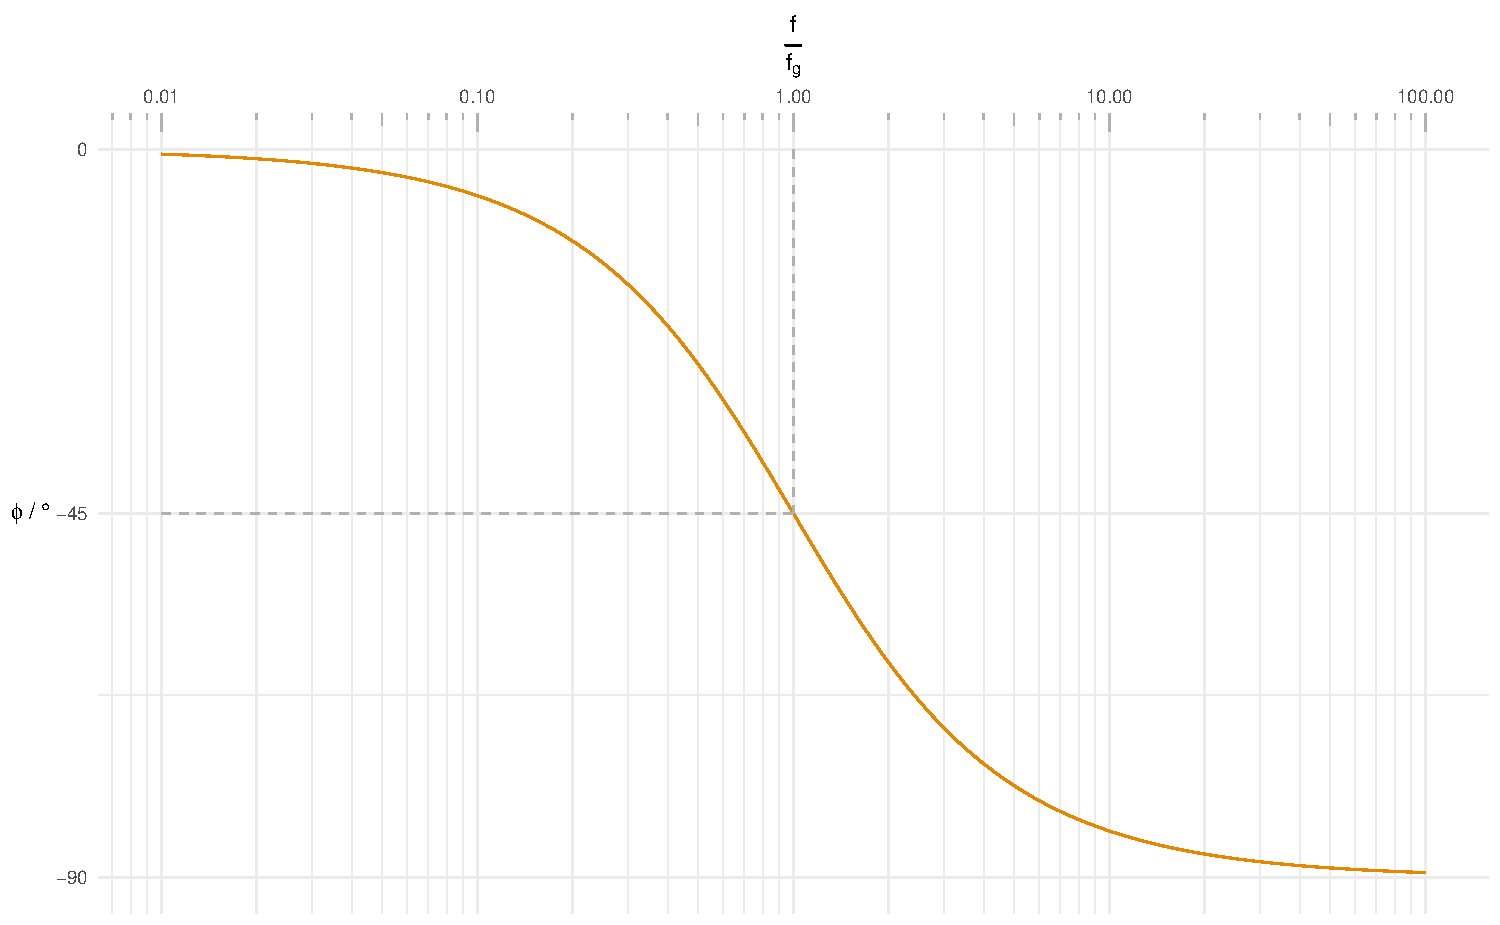
\includegraphics[scale=0.5]{./R/RC_LP/RC_LP_phase_clean.pdf}
        \end{center}

  \subsubsection*{RC-Hochpass}
    \begin{center}
      \begin{circuitikz}

        \draw (0,0) to[open,v^=$U_1$, o-o] (0,-3);
        \draw (.05,0) to[C, l=$C$] (4,0); % kinda hacked
        \draw (4,0) to[open] (6,0);
        \draw (4,0) -- (6,0);
        \draw (4,0) to[R, l=$R$, *-*] (4,-3);
        \draw (6,0) to[open,v^=$U_2$,o-o] (6,-3);
        \draw (5.95,-3) to[short] (0.05,-3);

      \end{circuitikz}
    \end{center}

    \begin{gather*}
      \frac{\underline{U}_2}{\underline{U}_1} = \frac{R}{R +\frac{1}{j \omega C}} = \frac{1}{1 - j \frac{1}{\omega R C}}\\
    \end{gather*}

    Amplitude:
      \begin{gather*}
        \frac{\mid \underline{U}_2 \mid}{\mid \underline{U}_1 \mid} = \frac{\mid 1 \mid}{\mid 1 - j \frac{1}{\omega R C} \mid} = \frac{1}{\sqrt{1 + \frac{1}{\omega^2 R^2 C^2}}}\\
      \end{gather*}

    Phase:
      \begin{gather*}
        \phi = \text{arg} \left( \frac{ \underline{U}_2 }{ \underline{U}_1 } \right) = 0 - \arctan{\left(-\frac{1}{\omega R C}\right)} = \arctan{ \frac{1}{\omega R C}}\\
      \end{gather*}

    Grenzfrequenz:
      \begin{gather*}
        \mid \text{Re}\left( \frac{ \underline{U}_2 }{ \underline{U}_1 } \right) \mid = \mid \text{Im}\left( \frac{ \underline{U}_2 }{ \underline{U}_1 } \right) \mid\\
        \text{Nach komplex-konjugierter Erweiterung:}\\
        \frac{1}{1 + \frac{1}{\omega_g^2 R^2 C^2}} = \frac{\frac{1}{\omega_g R C}}{1 + \frac{1}{\omega_g^2 R^2 C^2}}\\
      \end{gather*}

      \begin{gather*}
        \frac{1}{\omega_g R C} = 1\\
        \omega_g = \frac{1}{R C}
      \end{gather*}

    Normierung:
        \begin{gather*}
          \frac{\mid \underline{U}_2 \mid}{\mid \underline{U}_1 \mid} \left( \frac{\omega}{\omega_g} \right) = \frac{1}{\sqrt{1+\dfrac{1}{\left( \frac{\omega}{\omega_g} \right)^2} }} = \frac{1}{\sqrt{1+\dfrac{1}{\left(\frac{f}{f_g} \right)^2 }}}
        \end{gather*}

        \begin{gather*}
          \phi \left( \frac{\omega}{\omega_g} \right) = \arctan{ \frac{1}{\frac{\omega}{\omega_g}} }
        \end{gather*} \\

      Betragsgang: \\ \indent \indent siehe 1.5: Hochpassfilter\\\\
      \indent Phasengang:
        \begin{center}
          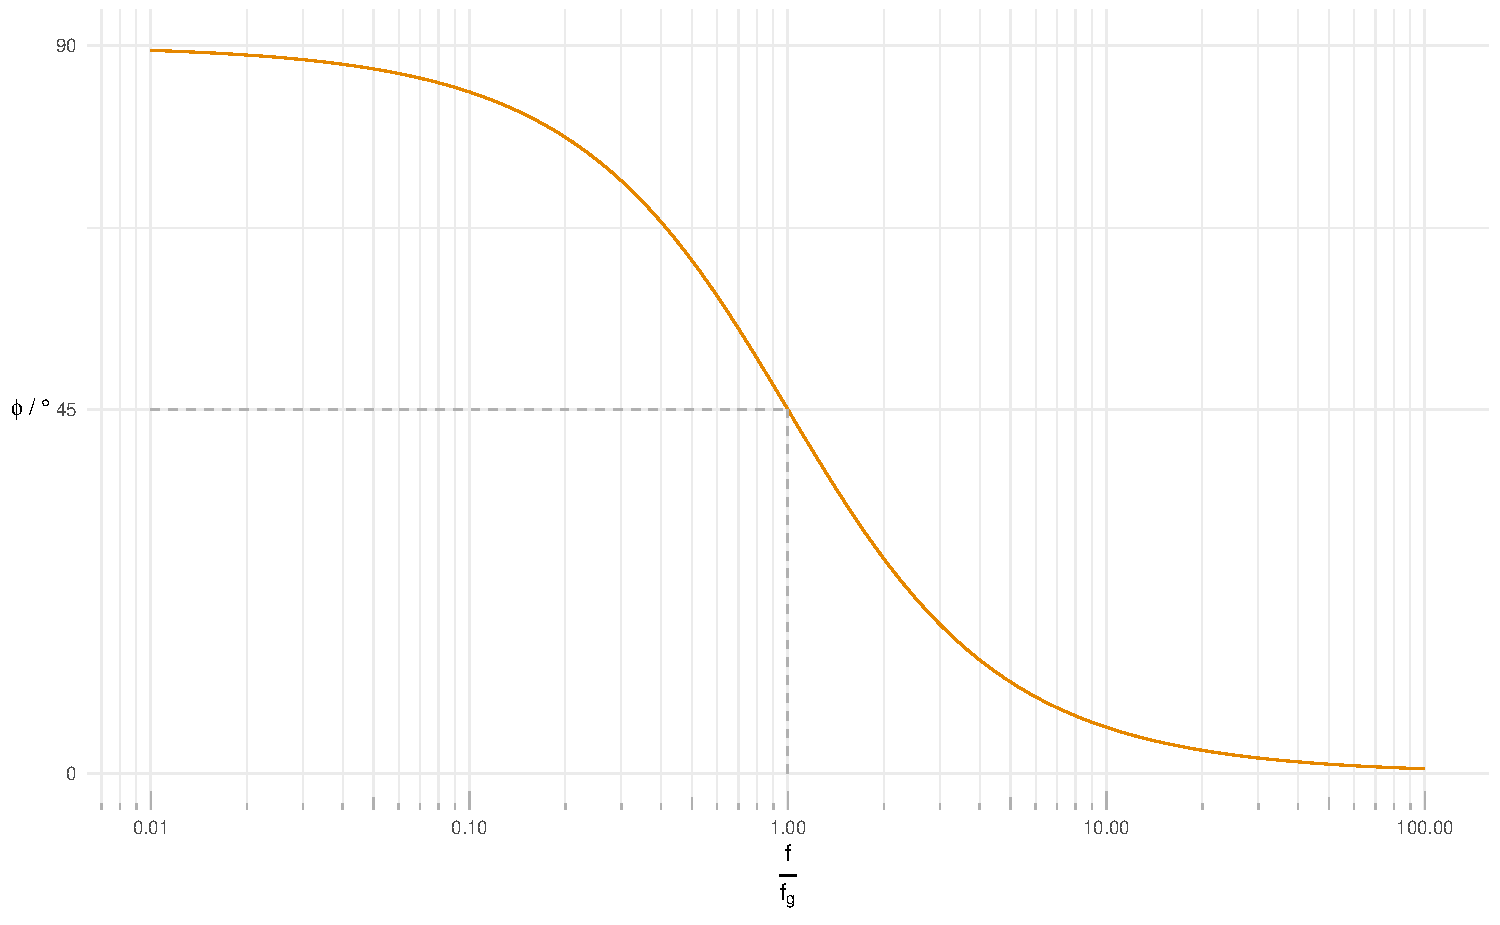
\includegraphics[scale=0.5]{./R/RL_HP/RL_HP_phase_clean.pdf}
        \end{center}

  \subsubsection*{RL-Tiefpass}

    \begin{center}
      \begin{circuitikz}

        \draw (0,0) to[open,v^=$U_1$, o-o] (0,-3);
        \draw (.05,0) to[L, l=$L$] (4,0); % kinda hacked
        \draw (4,0) to[open] (6,0);
        \draw (4,0) -- (6,0);
        \draw (4,0) to[R, l=$R$, *-*] (4,-3);
        \draw (6,0) to[open,v^=$U_2$,o-o] (6,-3);
        \draw (5.95,-3) to[short] (0.05,-3);

      \end{circuitikz}
    \end{center}

    \begin{gather*}
      \frac{\underline{U}_2}{\underline{U}_1} = \frac{R}{R+j \omega L} = \frac{1}{1 + j \frac{\omega L}{R}}\\
    \end{gather*}

    Amplitude:
      \begin{gather*}
        \frac{\mid \underline{U}_2 \mid}{\mid \underline{U}_1 \mid} = \frac{\mid 1 \mid}{\mid 1 + j \frac{\omega L}{R}\mid} = \frac{1}{\sqrt{1+ \frac{\omega^2 L^2}{R^2} }}\\
      \end{gather*}

    Phase:
      \begin{gather*}
        \phi = \text{arg} \left( \frac{ \underline{U}_2 }{ \underline{U}_1 } \right) = 0 - \arctan{\frac{ \frac{\omega L}{R} }{1}} = -\arctan{\left(\frac{\omega L}{R}\right)}\\
      \end{gather*}

    Grenzfrequenz:
      \begin{gather*}
        \mid \text{Re}\left( \frac{ \underline{U}_2 }{ \underline{U}_1 } \right) \mid = \mid \text{Im}\left( \frac{ \underline{U}_2 }{ \underline{U}_1 } \right) \mid\\
        \text{Nach komplex-konjugierter Erweiterung:}\\
        \frac{1}{1 + \dfrac{\omega_g^2 L^2}{R^2} } = \frac{ \frac{\omega_g L}{R} }{1 + \dfrac{\omega_g^2 L^2}{R^2} }\\
      \end{gather*}

      \begin{gather*}
        \frac{\omega_g L}{R} = 1\\
        \omega_g = \frac{R}{L}
      \end{gather*}

    Normierung:
      \begin{gather*}
        \frac{\mid \underline{U}_2 \mid}{\mid \underline{U}_1 \mid} \left( \frac{\omega}{\omega_g} \right) = \frac{1}{\sqrt{1+ \left (\dfrac{\omega}{\omega_g} \right)^2}} = \frac{1}{\sqrt{1+\left (\dfrac{f}{f_g} \right)^2}}
      \end{gather*}

      \begin{gather*}
        \phi \left( \frac{\omega}{\omega_g} \right) = -\arctan{ \frac{\omega}{\omega_g} }
      \end{gather*} \\

      Betragsgang: \\ \indent \indent siehe 1.5: Tiefpassfilter\\\\
      \indent Phasengang:
        \begin{center}
          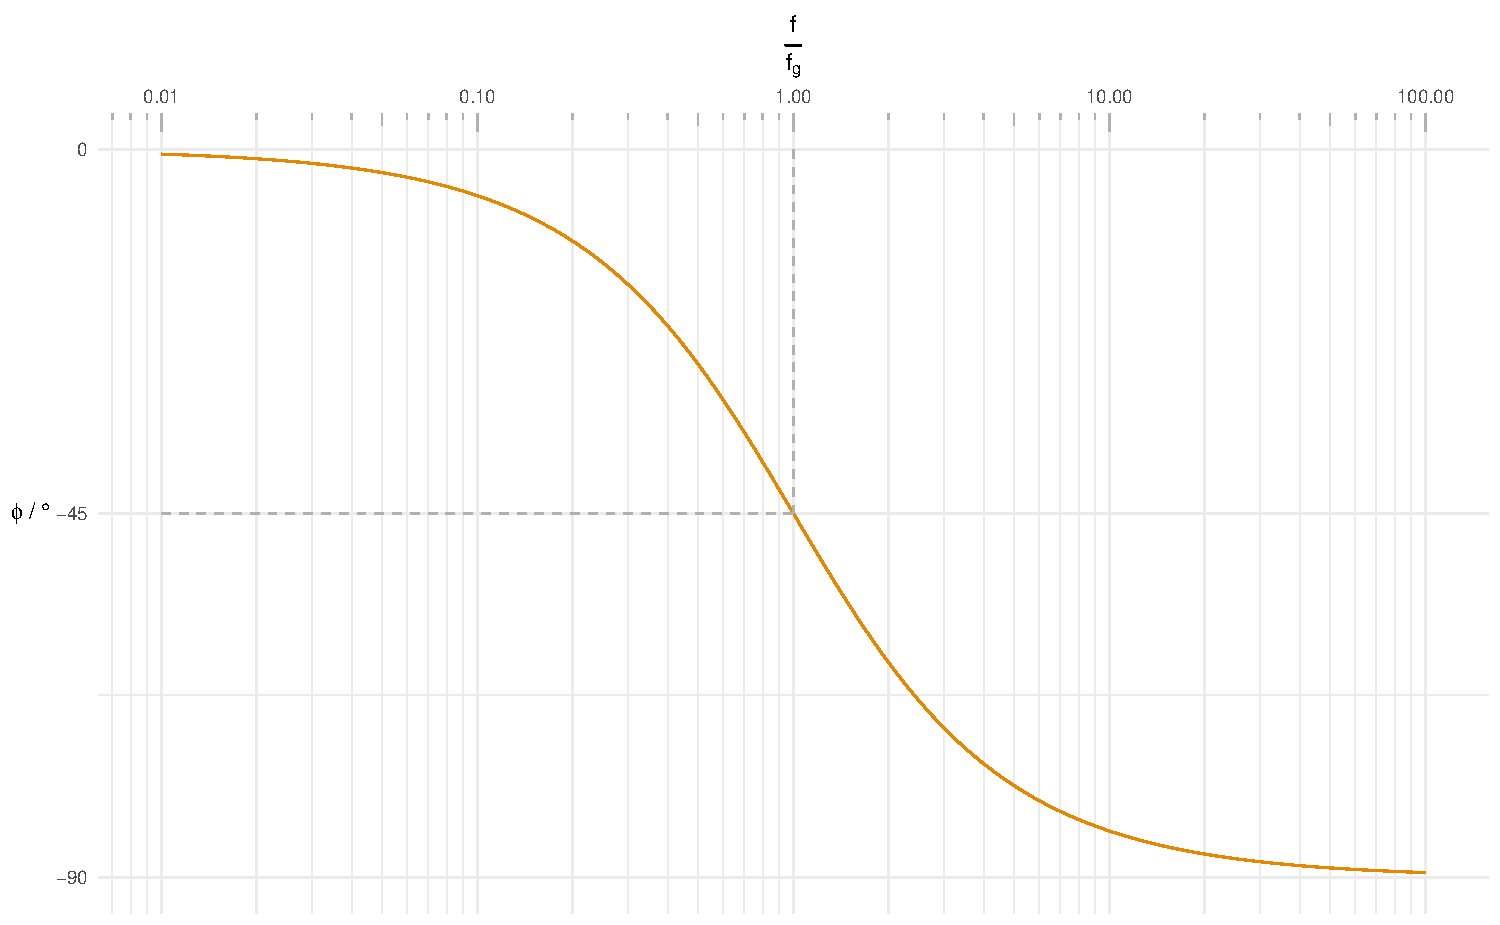
\includegraphics[scale=0.5]{./R/RC_LP/RC_LP_phase_clean.pdf}
        \end{center}

  \subsubsection*{RL-Hochpass}
    \begin{center}
      \begin{circuitikz}

        \draw (0,0) to[open,v^=$U_1$, o-o] (0,-3);
        \draw (.05,0) to[R, l=$R$] (4,0); % kinda hacked
        \draw (4,0) to[open] (6,0);
        \draw (4,0) -- (6,0);
        \draw (4,0) to[L, l=$L$, *-*] (4,-3);
        \draw (6,0) to[open,v^=$U_2$,o-o] (6,-3);
        \draw (5.95,-3) to[short] (0.05,-3);

      \end{circuitikz}
    \end{center}

    \begin{gather*}
      \frac{\underline{U}_2}{\underline{U}_1} = \frac{j \omega L}{R + j \omega L} = \frac{1}{1 - j \frac{R}{\omega L}}\\
    \end{gather*}

    Amplitude:
      \begin{gather*}
        \frac{\mid \underline{U}_2 \mid}{\mid \underline{U}_1 \mid} = \frac{\mid 1 \mid}{\mid 1 - j \frac{R}{\omega L} \mid} = \frac{1}{\sqrt{1 + \frac{R^2}{\omega^2 L^2}}}\\
      \end{gather*}

    Phase:
      \begin{gather*}
        \phi = \text{arg} \left( \frac{ \underline{U}_2 }{ \underline{U}_1 } \right) = 0 - \arctan{\left(-\frac{R}{\omega L}\right)} = \arctan{ \frac{R}{\omega L}}\\
      \end{gather*}

    Grenzfrequenz:
      \begin{gather*}
        \mid \text{Re}\left( \frac{ \underline{U}_2 }{ \underline{U}_1 } \right) \mid = \mid \text{Im}\left( \frac{ \underline{U}_2 }{ \underline{U}_1 } \right) \mid\\
        \text{Nach komplex-konjugierter Erweiterung:}\\
        \frac{1}{1 + \dfrac{R^2}{\omega_g^2 L^2}} = \frac{\frac{R}{\omega_g L}}{1+ \dfrac{R^2}{\omega_g^2 L^2}}\\
      \end{gather*}

      \begin{gather*}
        \frac{R}{\omega_g L} = 1\\
        \omega_g = \frac{R}{L}
      \end{gather*}

    Normierung:
      \begin{gather*}
        \frac{\mid \underline{U}_2 \mid}{\mid \underline{U}_1 \mid} \left( \frac{\omega}{\omega_g} \right) = \frac{1}{\sqrt{1+\dfrac{1}{\left( \frac{\omega}{\omega_g} \right)^2} }} = \frac{1}{\sqrt{1+\dfrac{1}{\left(\frac{f}{f_g} \right)^2 }}}
      \end{gather*}

      \begin{gather*}
        \phi \left( \frac{\omega}{\omega_g} \right) = \arctan{ \frac{1}{\frac{\omega}{\omega_g}} }
      \end{gather*} \\

      Betragsgang: \\ \indent \indent siehe 1.5: Hochpassfilter\\\\
      \indent Phasengang:
        \begin{center}
          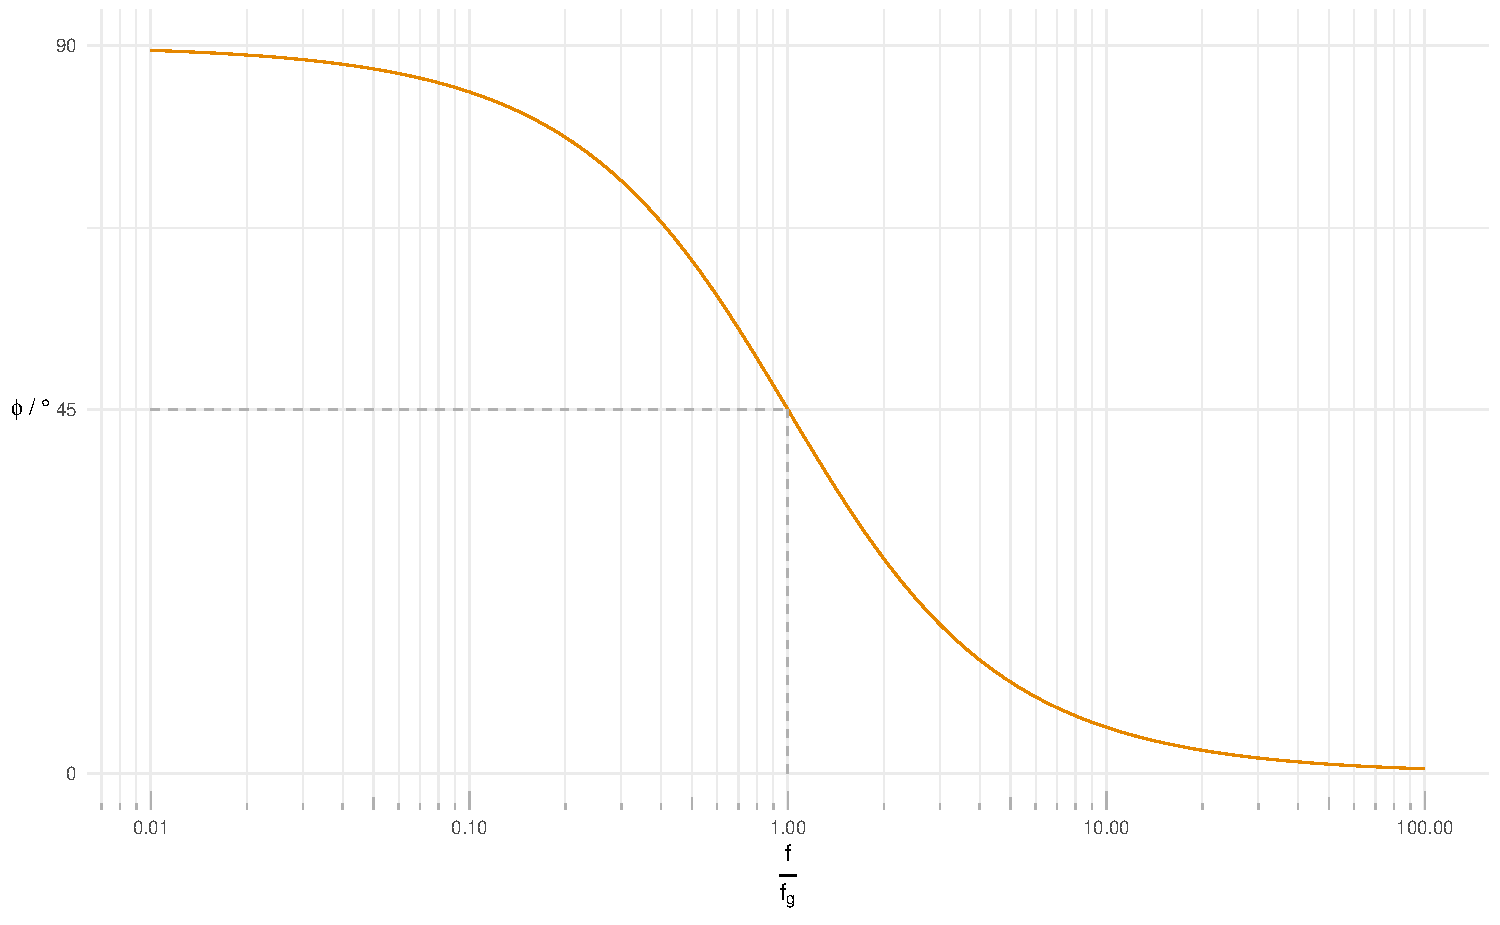
\includegraphics[scale=0.5]{./R/RL_HP/RL_HP_phase_clean.pdf}
        \end{center}

%1.7
\subsection{}
  \begin{center}
    \begin{circuitikz}

      \draw (0,0) to[open, v^=$U_1$, o-o] (0, -3);
      \draw (.05,0) to[R, l=$R_1$] (4,0); % kinda hacked
      \draw (4,0) to[open] (6,0);
      \draw (4,0) -- (6,0);
      \draw (4,0) to[L, l=$L$, *-*] (4,-3);
      \draw (4+2,0) to[R, l=$R_p$, *-*] (4+2,-3);
      \draw (4+4,0) to[C, l=$C$, *-*] (4+4,-3);
      \draw (10,0) to[open,v^=$U_2$,o-o] (10,-3);
      \draw (9.95,-3) to[short] (0.05,-3);
      \draw (4,0) to[short] (9.95, 0);

    \end{circuitikz}

  \end{center}

  $$ R_1 = 1 \,\ \si{\kilo\ohm} \text{, } R_p = 1 \,\ \si{\kilo\ohm} \text{, }  L = 1 \,\ \si{\milli\henry} \text{, }  C = 1 \,\ \si{\micro\farad}$$

  \begin{gather*}
    \underline{Z} = R_1 + \dfrac{1}{j \omega C + \dfrac{1}{\omega L} + \dfrac{1}{R_p}}\\
    \frac{\underline{U_2}}{\underline{U_1}} = \dfrac{\dfrac{1}{j \omega C + \dfrac{1}{\omega L} + \dfrac{1}{R_p}}}{R_1 + \dfrac{1}{j \omega C + \dfrac{1}{\omega L} + \dfrac{1}{R_p}}} = \frac{1}{j R_1 \omega C + \dfrac{R_1}{j \omega L} + \dfrac{R_1}{R_p} + 1}\\\\
    \frac{\underline{U_2}}{\underline{U_1}} = \frac{1}{1+ \dfrac{R_1}{R_p} + j \left (\omega R_1 C - \dfrac{R_1}{\omega L} \right)}
  \end{gather*}

  Grenzfrequenzen:
    \begin{align*}
      \mid \text{Re}\left( \frac{ \underline{U}_2 }{ \underline{U}_1 } \right) \mid &= \mid \text{Im}\left( \frac{ \underline{U}_2 }{ \underline{U}_1 } \right) \mid\\
      R_1 \left(\omega_{\pm 45} C - \frac{1}{\omega_{\pm 45} L} \right) &= 1 + \frac{R_1}{R_p}\\
      \omega_{\pm 45} C - \frac{1}{\omega_{\pm 45} L} &= \frac{1}{R_1} + \frac{1}{R_p}\\
      \frac{1}{\omega_{\pm 45}}\left( \omega_{\pm 45}^2 C - \frac{1}{L} \right) &= \frac{R_1+R_p}{R_1 \cdot R_p}\\
      \omega_{\pm 45}^2 C - \frac{1}{L} &= \omega_{\pm 45} \frac{R_1+R_p}{R_1 \cdot R_p}
    \end{align*}

    \begin{gather*}
      \omega_{\pm 45}^2 - \omega_{\pm 45} \frac{R_1+R_p}{C \cdot R_1 \cdot R_p} - \frac{1}{LC} = 0\\\\
      \omega_{\pm 45} = \sqrt{\left( \frac{R_1 + R_p}{2 \cdot C R_1 R_p}\right)^2 + \frac{1}{LC}} \pm \frac{R_1+R_p}{2\cdot C R_1 R_p}\\\\
      \text{Mit den Beispielwerten:}\\
      \omega_{\pm 45} = \sqrt{\left( \frac{1 \si{\kilo\ohm} + 1 \si{\kilo\ohm}}{2 \cdot 1 \si{\micro\farad} \cdot 1 \si{\kilo\ohm} \cdot 1 \si{\kilo\ohm}}\right)^2 + \frac{1}{1 \si{\milli\henry} \cdot 1 \si{\micro\farad}}} \pm \frac{1 \si{\kilo\ohm}+1 \si{\kilo\ohm}}{2\cdot 1 \si{\micro\farad} \cdot 1 \cdot \si{\kilo\ohm} \cdot 1 \si{\kilo\ohm}}\\
      \omega_{+45} = 32638.584 \,\ \si{s}^{-1} \text{, } f_{+45} = 5194.592 \,\ \si{Hz}\\
      \omega_{-45} = 30638.584 \,\ \si{s}^{-1} \text{, } f_{+45} = 4876.282 \,\ \si{Hz}\\
      B_{\omega}   = \omega_{+45} - \omega_{-45} = 2000 \,\ \si{s}^{-1}\\
      B_{f}        = 318.31 \si{Hz}
    \end{gather*}

  Resonanzfrequenz:
    \begin{gather*}
      \text{Im}\left( \frac{ \underline{U}_2 }{ \underline{U}_1 } \right) = 0\\
      \frac{\omega_0 R_1 C - \frac{R_1}{\omega_0 L}}{\left( 1+\frac{R_1}{R_p} \right)^2 + \left( \omega_0 R_1 C - \frac{R_1}{\omega_0 L}\right)^2} = 0\\
      \omega_0 R_1 C = \frac{R_1}{\omega_0 L}\\
      \omega_0^2 = \frac{1}{LC}\\
      \omega_0 = \frac{1}{\sqrt{LC}} = \frac{1}{\sqrt{1 \si{\milli\henry} \cdot 1 \si{\micro\farad}}}=31622.777 \,\ \si{s}^{-1}\\
      f_0 = 5032.921 \si{Hz}\\
    \end{gather*}

  Betrag:
    \begin{gather*}
      \frac{\mid \underline{U}_2 \mid}{\mid \underline{U}_1 \mid} = \frac{1}{  \sqrt{ \left( 1+ \dfrac{R_1}{R_p} \right)^2  + R_1^2 \left( \omega C - \dfrac{1}{\omega L} \right)^2}}\\
    \end{gather*}

  Betrag bei Resonanzfrequenz:
    \begin{align*}
      \frac{\mid \underline{U}_2 \mid}{\mid \underline{U}_1 \mid} \left( \omega = \omega_0 \right) &= \frac{1}{ \sqrt{ \left( 1+ \dfrac{R_1}{R_p} \right)^2  + R_1^2 \left( \frac{1}{\sqrt{LC}} C - \dfrac{1}{\frac{1}{\sqrt{LC}} L} \right)^2}}\\
      &= \frac{1}{ \sqrt{ \left( 1+ \dfrac{R_1}{R_p} \right)^2  + R_1^2 \left( \frac{LC-\sqrt{LC}^2}{\sqrt{LC}L} \right)^2}} = \frac{1}{1+\dfrac{R_1}{R_p}} = \frac{R_p}{R_1+R_p}\\
    \end{align*}

    \begin{gather*}
      \text{Mit den Beispielwerten:}\\
      \frac{\mid \underline{U}_2 \mid}{\mid \underline{U}_1 \mid} \left( \omega = \omega_0 \right) = \frac{1 \si{\kilo\ohm}}{1 \si{\kilo\ohm} + \si{\kilo\ohm}} = \frac{1}{2}\\
      \frac{\mid \underline{U}_2 \mid}{\mid \underline{U}_1 \mid} \left( \omega = \omega_{\pm 45} \right) = \frac{R_p}{R_1+R_p} \cdot \frac{1}{\sqrt{2}} = \frac{1}{2} \cdot \frac{1}{\sqrt{2}} = \frac{1}{\sqrt{8}}
    \end{gather*}

    %\vspace{0.021276873\paperheight}
    \begin{center}
      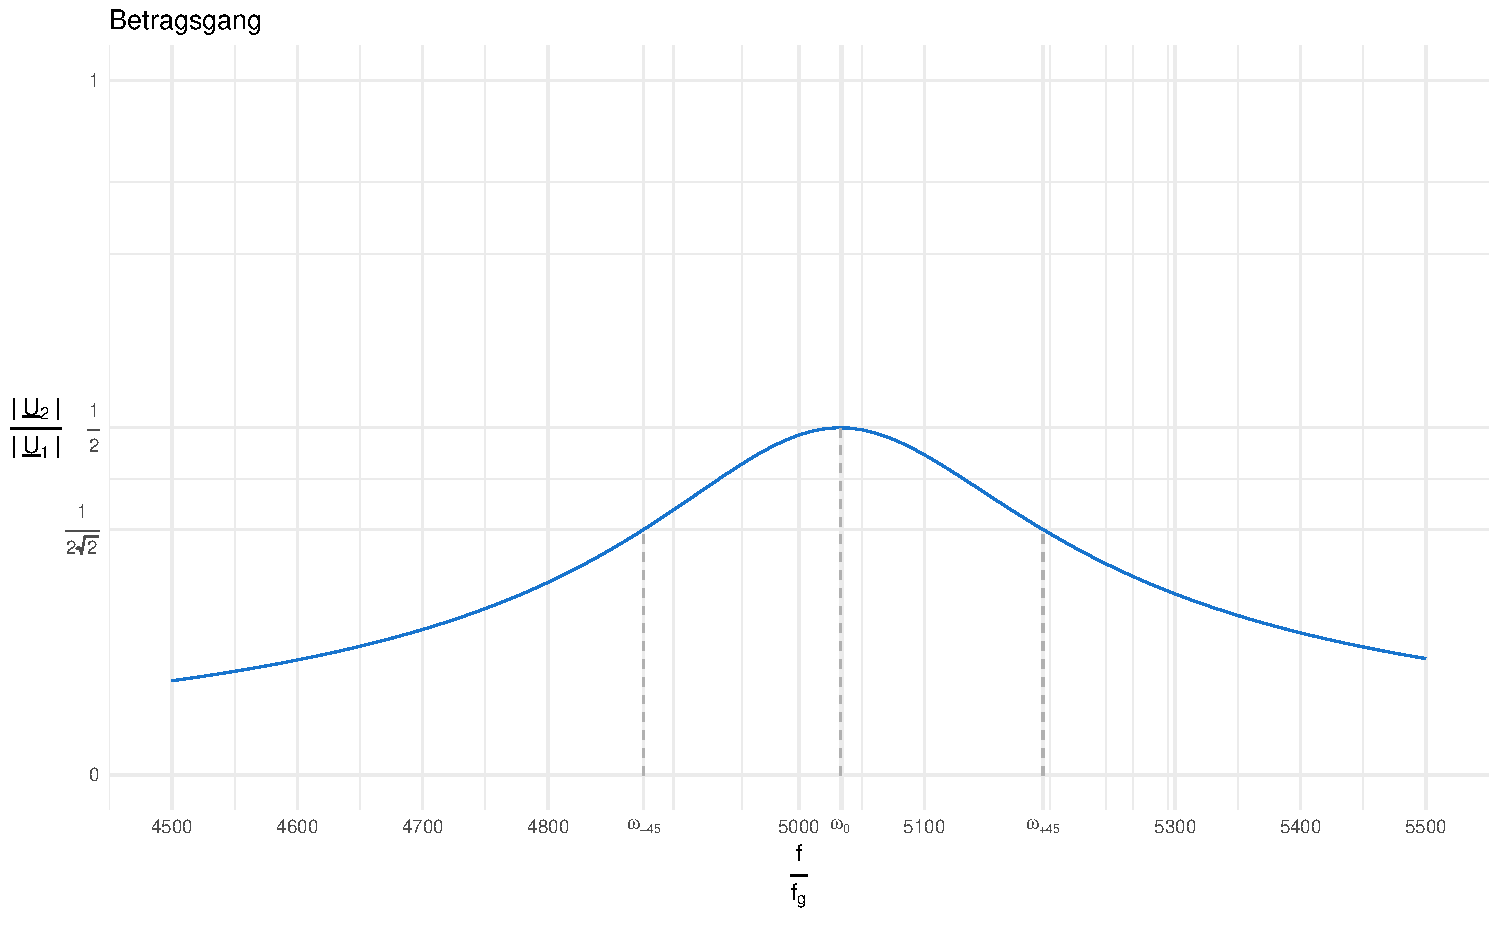
\includegraphics[scale=0.5]{./R/2_7/2_7_betrag_clean.pdf}
    \end{center}

  Phase:
    \begin{gather*}
      \phi = 0 - \arctan{\left( \frac{\omega R_1 C - \dfrac{R_1}{\omega L}}{1+ \dfrac{R_1}{R_p}} \right)} = -\arctan{\left( \frac{\omega C - \dfrac{1}{\omega L}}{\dfrac{1}{R_1}+ \dfrac{1}{R_p}} \right)}
    \end{gather*}
    \vspace{0.021276873\paperheight}
    \begin{center}
      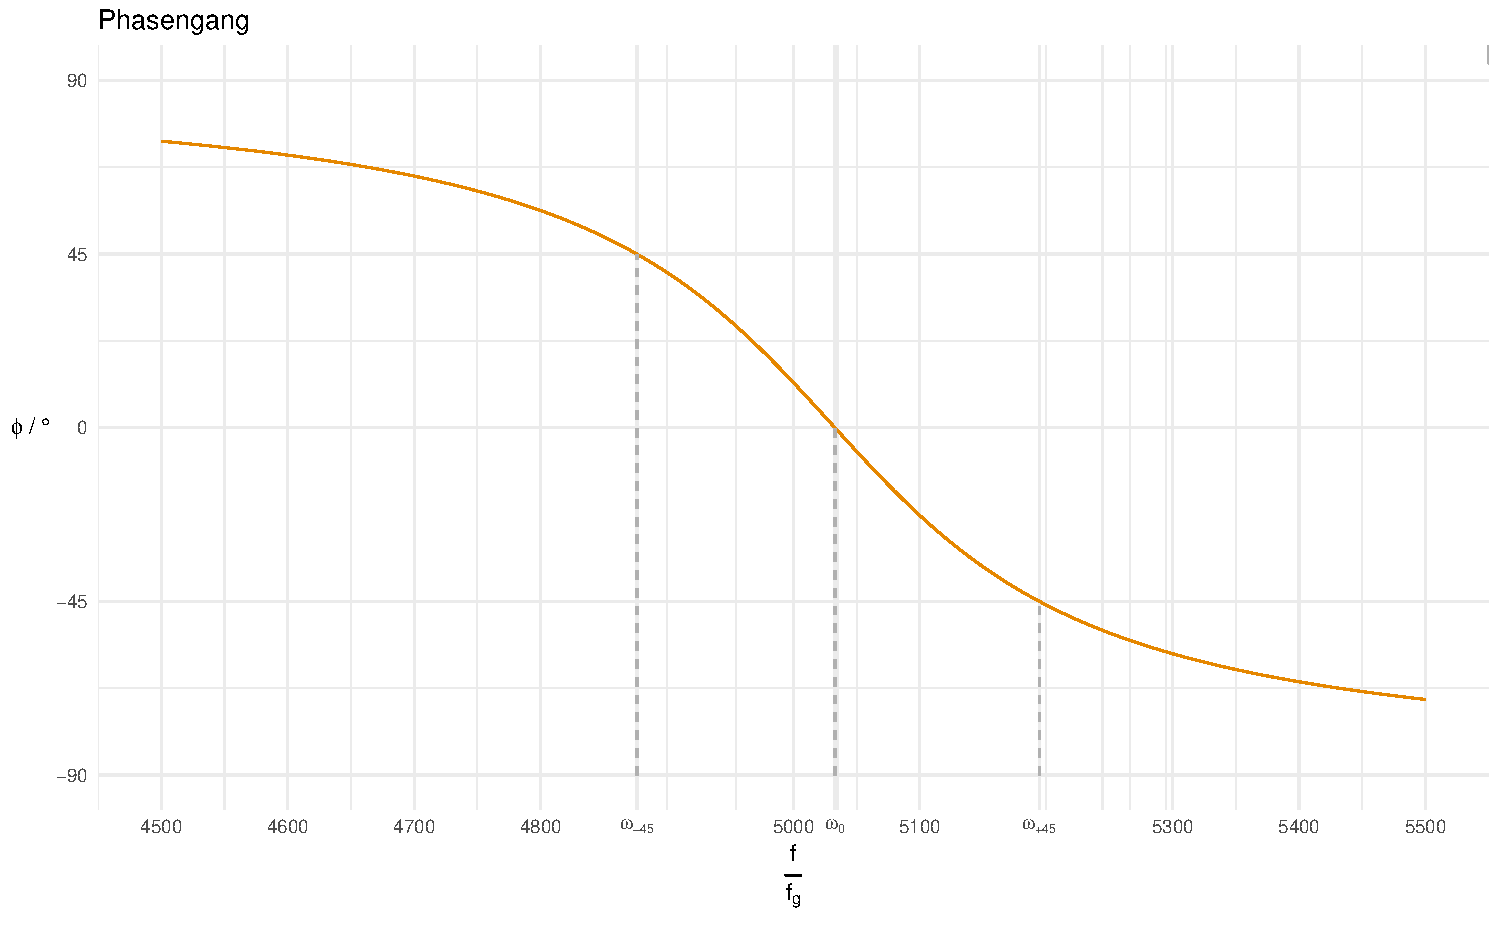
\includegraphics[scale=0.5]{./R/2_7/2_7_phase_clean.pdf}
    \end{center}

\pagebreak
\section{Versuchsaufgaben}
    Alle Messungen von Spannung, Frequenz sowie Phase erfolgten mithilfe eines digitalen Oszilloskops; alle Messungen von Bauteilkenngrößen mithilfe eines LCR-Meters.\\
  %2.1
  \subsection{RC-Tiefpass}

    \begin{table}[H]
    \begin{center}
    \begin{tabular}{|c|c|c|c|}
    \hline
    $\dfrac{f}{f_g}$  & $ \mid \underline{U_1} \mid / \si{\volt}$   & $\mid \underline{U_2} \mid / \si{\volt}$    & $\phi / \degree$ \\
    \hline
    0.01 & 1.02 & 1     & -1.3  \\
    0.1  & 1.02 & 1     & -5.6  \\
    0.2  & 1.02 & 0.98  & -11.2 \\
    0.3  & 1.01 & 0.95  & -16.7 \\
    0.4  & 1.01 & 0.92  & -22.8 \\
    0.5  & 1.01 & 0.9   & -27.4 \\
    0.8  & 1.01 & 0.79  & -39.8 \\
    1    & 1.01 & 0.71  & -45.7 \\
    2    & 0.99 & 0.45  & -63   \\
    4    & 0.99 & 0.25  & -76.1 \\
    7    & 0.99 & 0.15  & -83   \\
    10   & 0.99 & 0.11  & -86   \\
    30   & 0.99 & 0.036 & -89   \\
    100  & 1.01 & 0.01  & -99   \\
    \hline
    \end{tabular}
    \end{center}
    \caption*{Messwerte aus Aufgabe 4.1}
    \end{table}

    \noindent Am verwendeten Tiefpassfilter wurden die folgenden Kenngrößen gemessen:\\
    \vspace{0.4cm}
    $R = 6 \,\ \si{\kilo\ohm}$,
    $C = 4.4 \,\ \si{\nano\farad}$.\\\\
    Daraus ließ sich die Grenzfrequenz rechnerisch ermitteln:
    $$ f_g = \frac{1}{2 \pi R C} = \frac{1}{ 2 \pi \cdot 6 \si{\kilo\ohm} \cdot 4.4 \si{\nano\farad}} \approx 6.03 \,\ \si{\kilo\hertz}$$

    \noindent Die Grenzfrequenz wurde dann auch durch Einstellen der Frequenz und gleichzeitiger Messung des Phasenwinkels zu $-45 \degree$ gemessen:
    $$f_{g_{gemessen}} = 5.902 \,\ \si{\kilo\hertz}$$

    \noindent Zur Bildung der Verhältnisse $\frac{f}{f_g}$ für die Messreihe wurde die berechnete Grenzfrequenz verwendet.\\

    \noindent Die folgenden Diagramme zeigen die Messwerte (rosa) im Vergleich zum theoretischen Verlauf (blau/orange).\\

    \begin{center}
      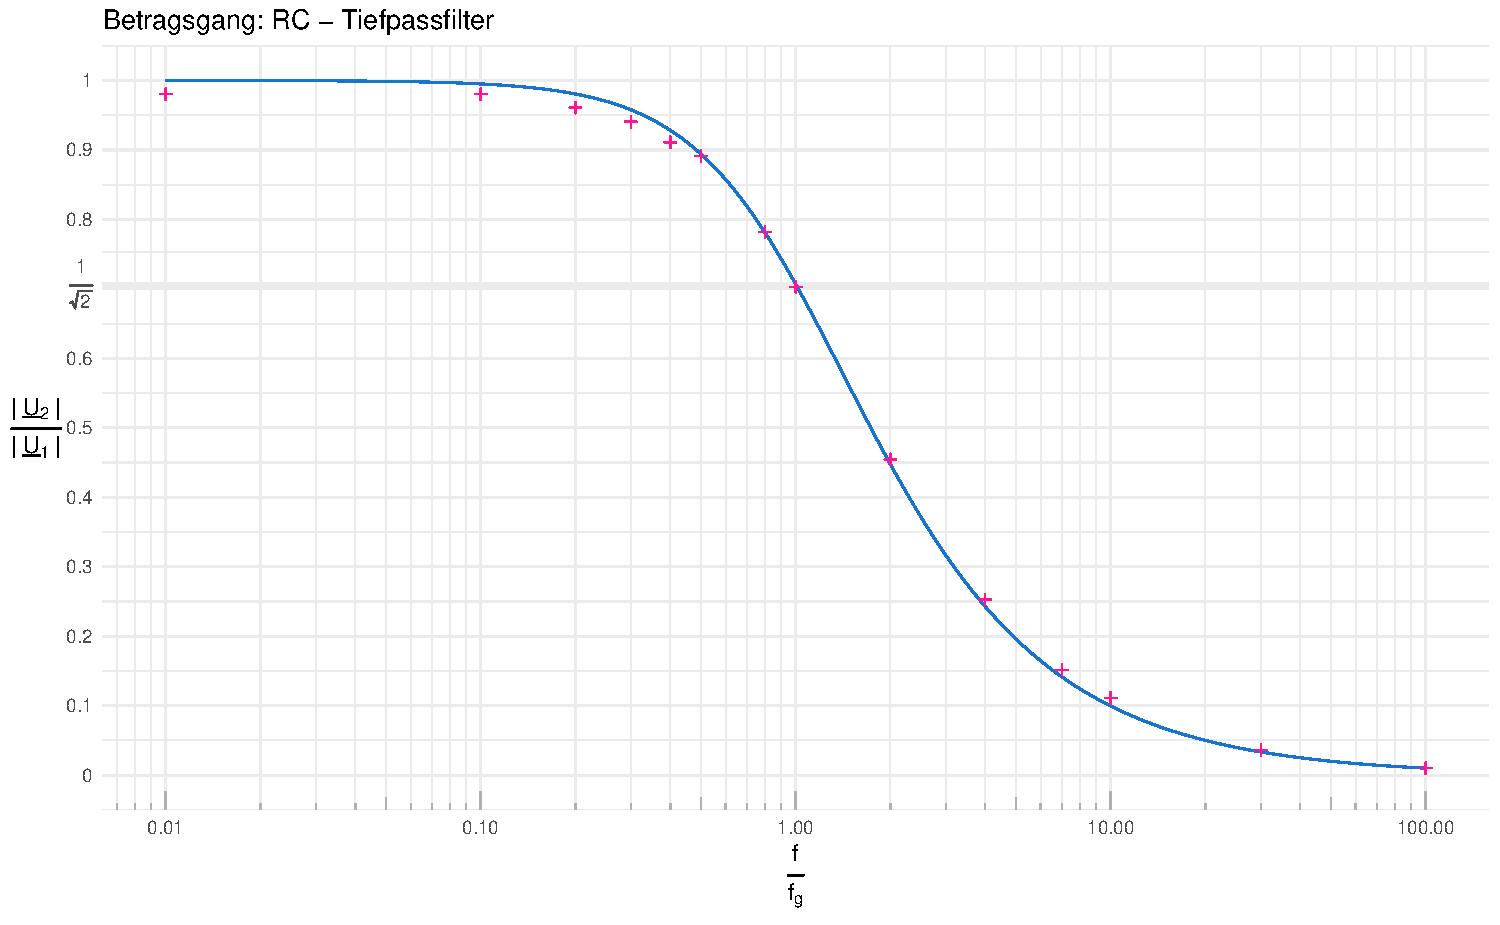
\includegraphics[scale=0.5]{./R/RC_LP/RC_LP.pdf}
      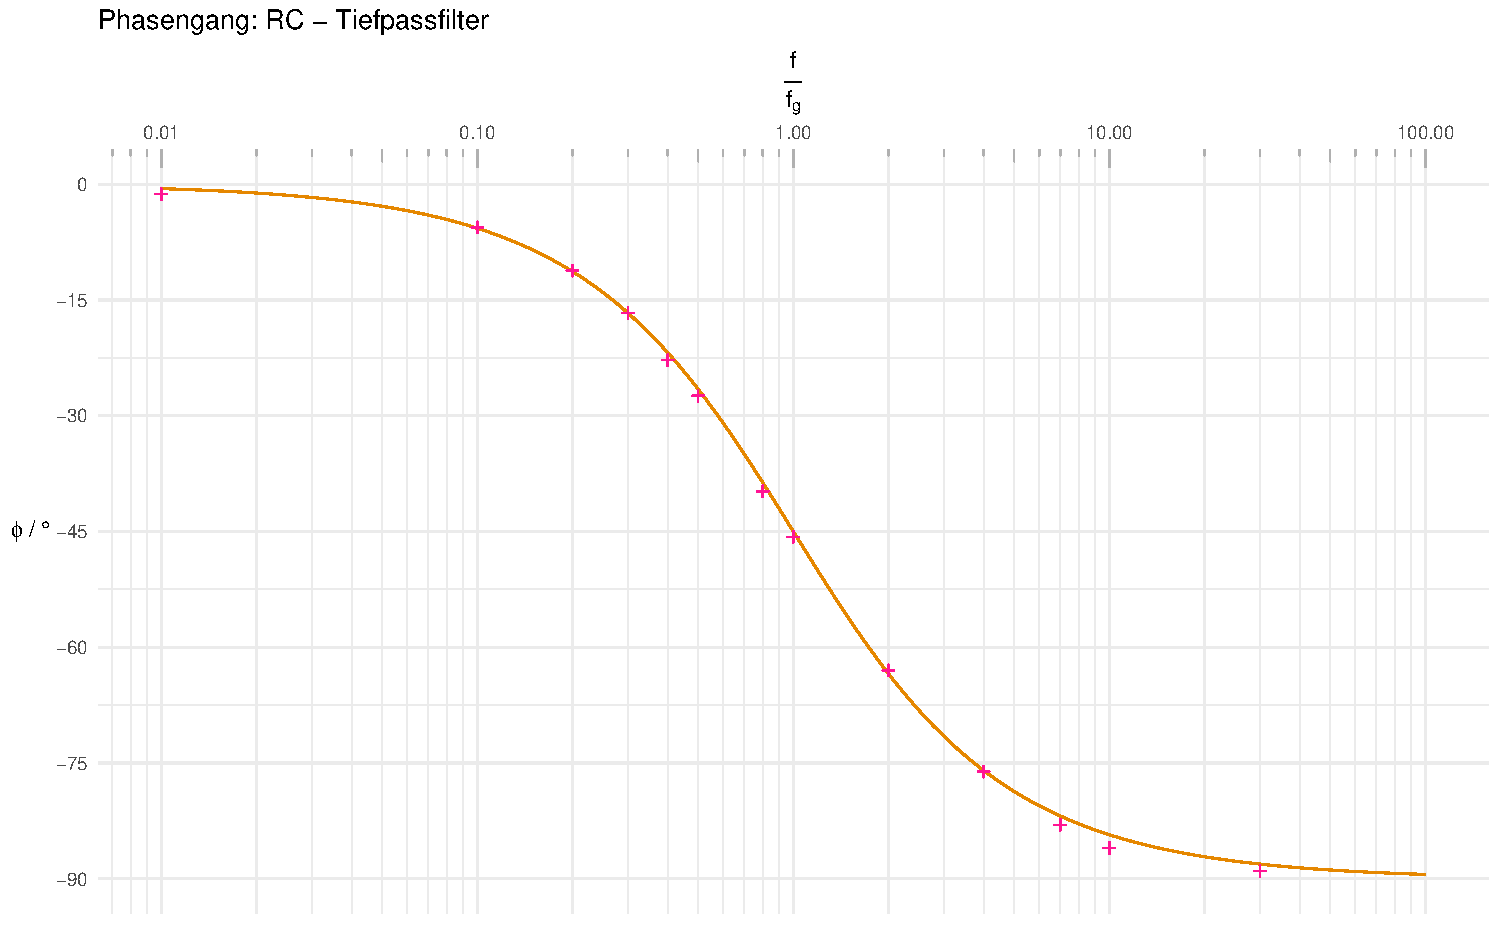
\includegraphics[scale=0.5]{./R/RC_LP/RC_LP_phase.pdf}
    \end{center}


  \subsection{RL-Hochpass}
    \begin{table}[H]
    \begin{center}
    \begin{tabular}{|c|c|c|c|}
    \hline
    $\dfrac{f}{f_g}$  & $ \mid \underline{U_1} \mid / \si{\volt}$   & $\mid \underline{U_2} \mid / \si{\volt}$    & $\phi / \degree$ \\
    \hline
    0.01 & 1.01 & 0.0145 & 80    \\
    0.05 & 1.03 & 0.05   & 83    \\
    0.1  & 1.03 & 0.0975 & 81    \\
    0.2  & 1.03 & 0.201  & 76    \\
    0.4  & 1.03 & 0.378  & 66.8  \\
    0.7  & 1.03 & 0.58   & 53.5  \\
    1    & 1.03 & 0.7    & 44.5  \\
    2    & 1.01 & 0.92   & 25    \\
    4    & 1.01 & 1      & 11.1  \\
    7    & 1.02 & 1.01   & 3.4   \\
    \hline
    \end{tabular}
    \end{center}
    \caption*{Messwerte aus Aufgabe 4.2}
    \end{table}

    \noindent Am verwendeten Hochpassfilter wurden die folgenden Kenngrößen gemessen:\\
    \vspace{0.4cm}
    $R = 3.23 \,\ \si{\kilo\ohm}$,
    $L = 102.35 \,\ \si{\milli\henry}$.\\\\
    Daraus ließ sich die Grenzfrequenz rechnerisch ermitteln:
    $$ f_g = \frac{R}{2 \pi L} = \frac{3.23 \si{\kilo\ohm}}{ 2 \pi \cdot 102.35 \si{\milli\henry}} \approx 5.02218 \,\ \si{\kilo\hertz}$$

    \noindent Die Grenzfrequenz wurde dann auch durch Einstellen der Frequenz und gleichzeitiger Messung des Phasenwinkels zu $45 \degree$ gemessen:
    $$f_{g_{gemessen}} = 5.020 \,\ \si{\kilo\hertz}$$

    \noindent Zur Bildung der Verhältnisse $\frac{f}{f_g}$ für die Messreihe wurde die gemessene Grenzfrequenz verwendet.\\

    \noindent Die folgenden Diagramme zeigen die Messwerte (rosa) im Vergleich zum theoretischen Verlauf (blau/orange).\\

    \begin{center}
      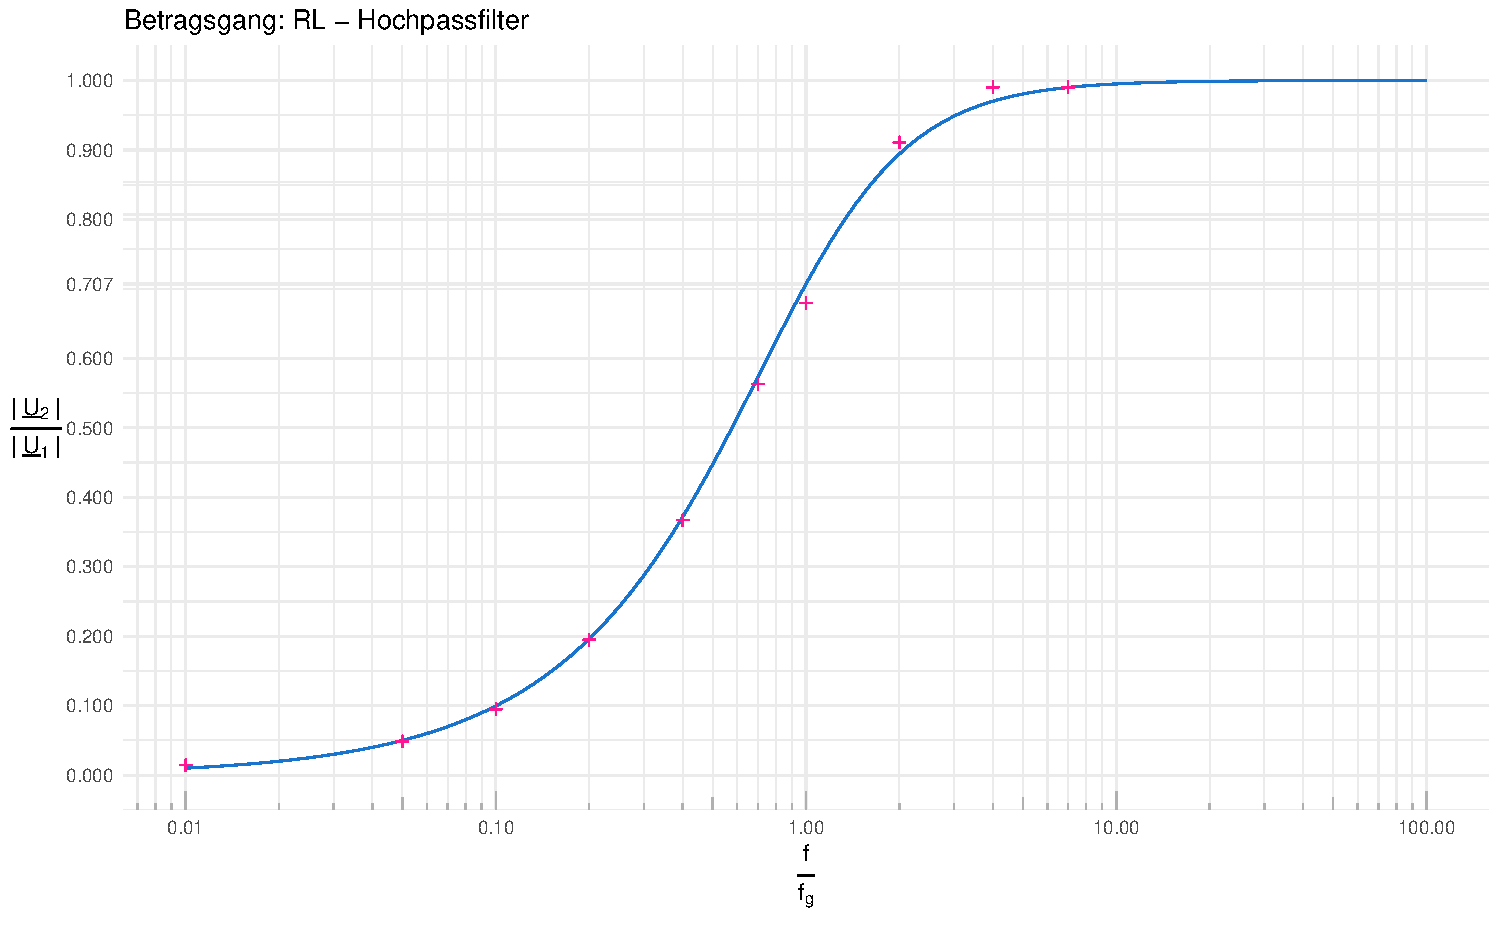
\includegraphics[scale=0.5]{./R/RL_HP/RL_HP.pdf}
    \end{center}

    \begin{center}
      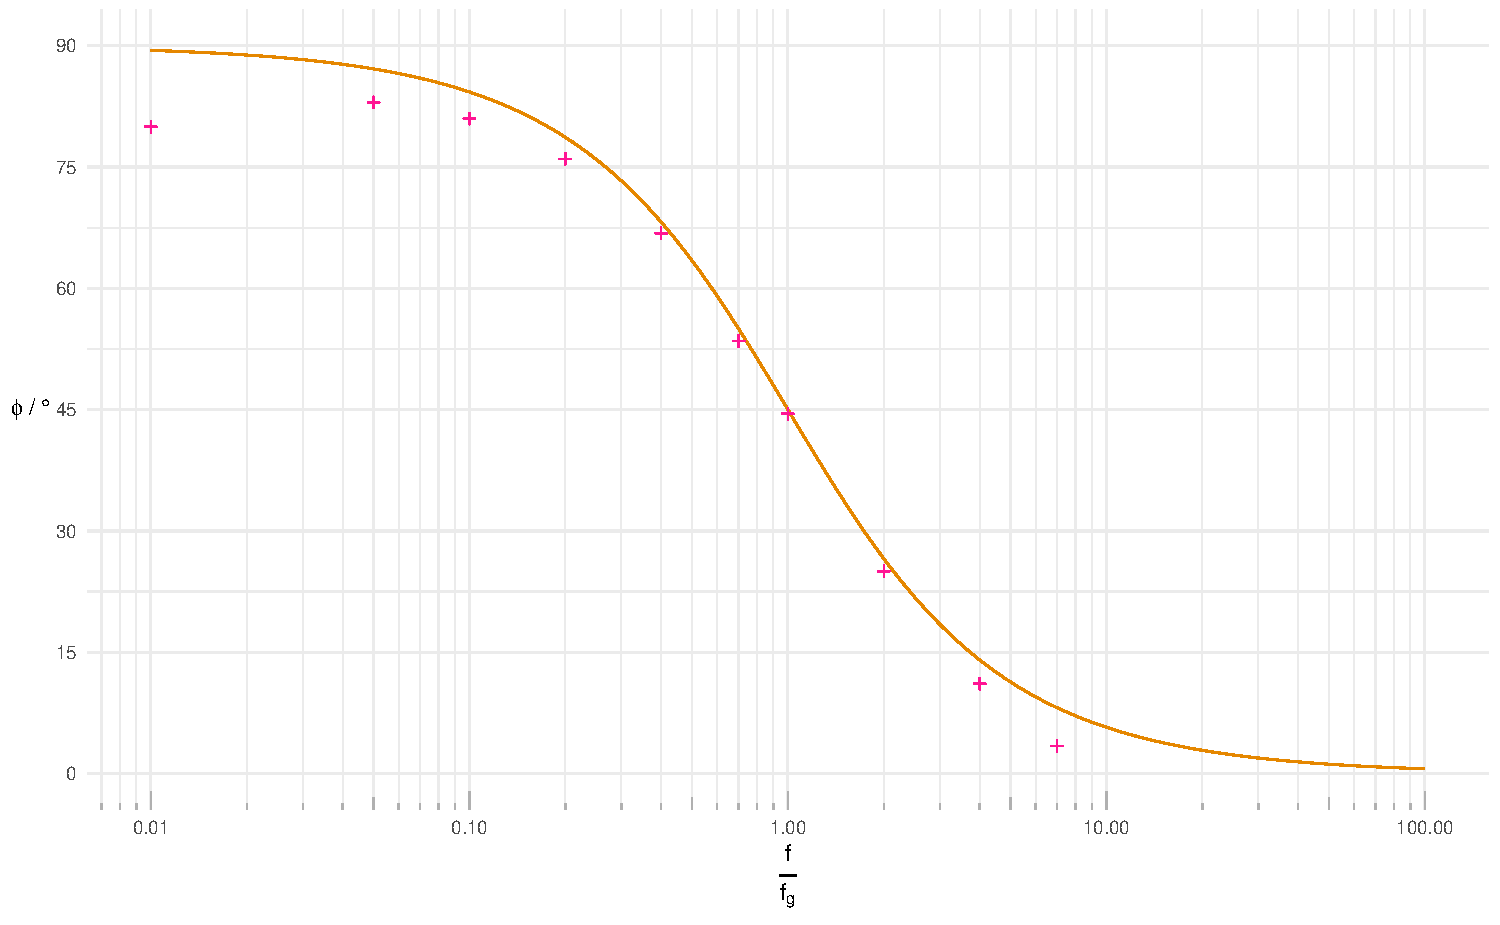
\includegraphics[scale=0.5]{./R/RL_HP/RL_HP_phase.pdf}
    \end{center}

    Bemerkung: Ab der Messung für $\frac{f}{f_g} = 10$ wurde diese ungenau. Es wurde ein negativer Winkel gemessen, was von den mit steigender Frequenz zunehmenden parasitären Eigenschaften (kapazitiv) der Anordnung zeugt.

  \subsection{RLC-Netzwerk}

    \begin{table}[H]
    \begin{center}
    \begin{tabular}{|l|l|l|l|}
    \hline
    $f / \si{\hertz}$  & $ \mid \underline{U_1} \mid / \si{\volt}$   & $\mid \underline{U_2} \mid / \si{\volt}$ & $\phi / \degree$ \\
    \hline
    3000 & 0.97 & 0.031 & 80    \\
    4000 & 0.97 & 0.066 & 74.8  \\
    4500 & 0.97 & 0.123 & 62.6  \\
    4700 & 0.96 & 0.179 & 52    \\
    4800 & 0.96 & 0.23  & 41    \\
    4900 & 0.98 & 0.265 & 27.3  \\
    5000 & 0.98 & 0.297 & 8     \\
    5036 & 0.98 & 0.302 & 0.3   \\
    5100 & 0.98 & 0.297 & -13   \\
    5200 & 0.98 & 0.265 & -31.2 \\
    5300 & 0.97 & 0.223 & -44.8 \\
    5500 & 0.96 & 0.159 & -59.9 \\
    5600 & 0.97 & 0.09  & -76.1 \\
    5700 & 0.96 & 0.047 & -82.6 \\
    \hline
    \end{tabular}
    \end{center}
    \caption*{Messwerte der Aufgabe 4.3}
    \end{table}

    \noindent Das Amplitudenverhältnis sowie die Phase des RLC-Netzwerks wurden für Frequenzen im Intervall $ 3 \,\ \si{\kilo\hertz}$ bis $ 5.7\,\ \si{\kilo\hertz}$ gemessen.\\

    \noindent Die gemessenen Grenzfrequenzen sind:\\
    $f_{+45} = 5.304 \,\ \si{\kilo\hertz}$\\
    $f_{-45} = 4.768 \,\ \si{\kilo\hertz}$\\\\
    Die daraus resultierende Bandbreite ist: (theoretisch: 318.31 Hz)\\
    $B_f = (5.304 - 4.768) \si{\kilo\hertz} = 536 \,\ \si{\hertz}$\\\\

    \noindent Dies entspricht einer Abweichung von etwa $-2.2\%$ von den theoretischen Werten der Grenzfrequenzen (siehe 1.7)\\

    \noindent Die gemessene Resonanzfrequenz ist: (theoretisch: 5.033 kHz)\\
    $f_0 = 5.036 \,\ \si{\kilo\hertz}$\\\\


    \noindent Die folgenden Diagramme zeigen die Messwerte (rosa) im Vergleich zum theoretischen Verlauf (blau/orange).\\

    \begin{center}
      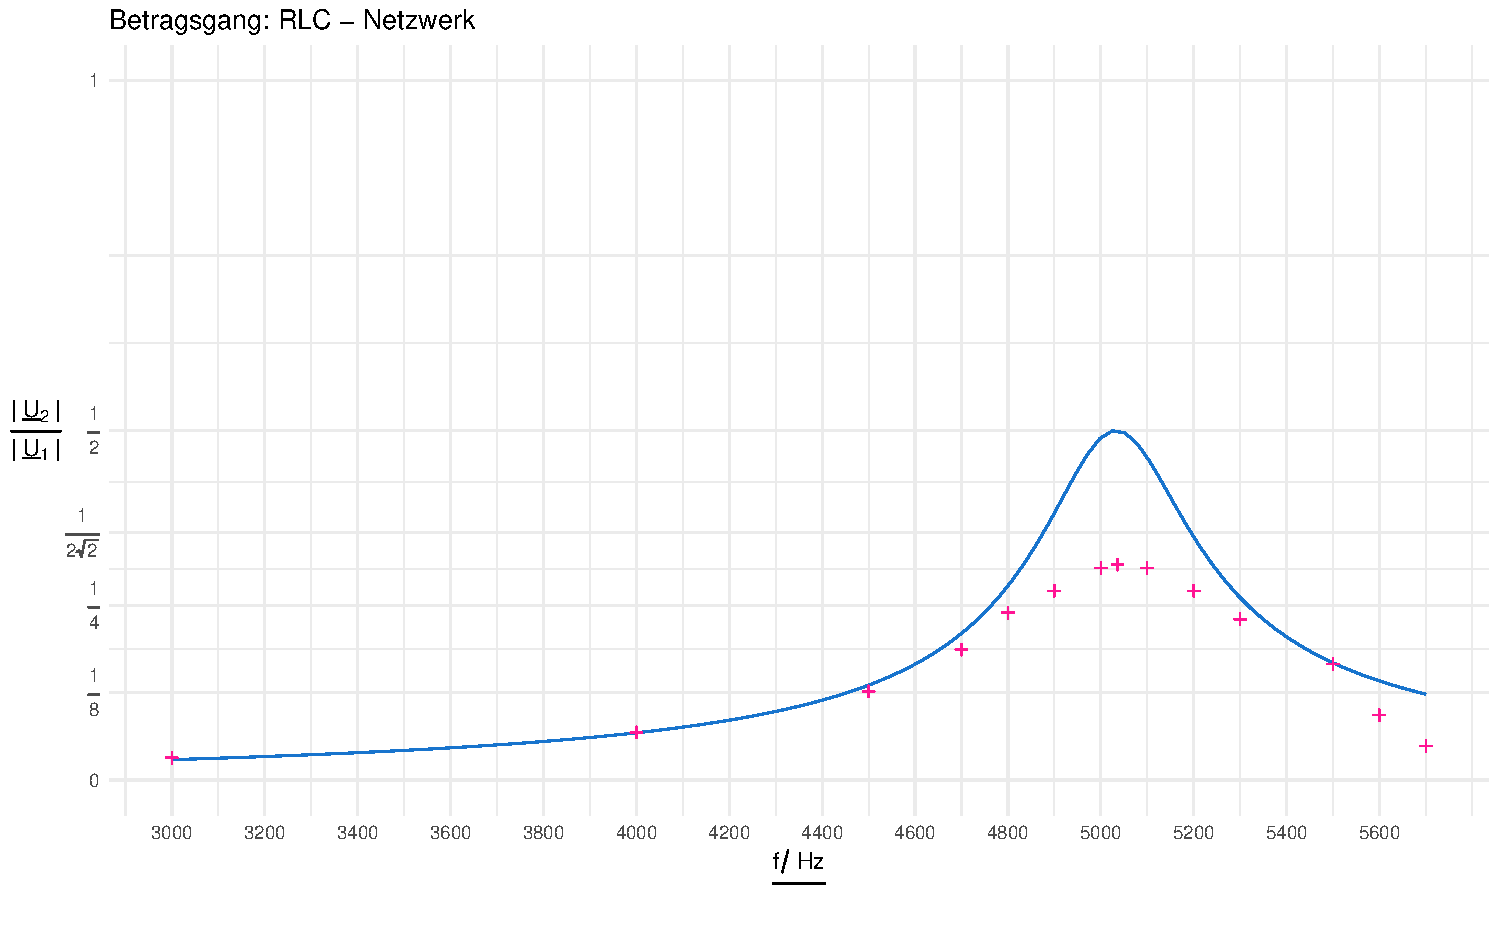
\includegraphics[scale=0.5]{./R/2_7/2_7_betrag.pdf}
    \end{center}

    \begin{center}
      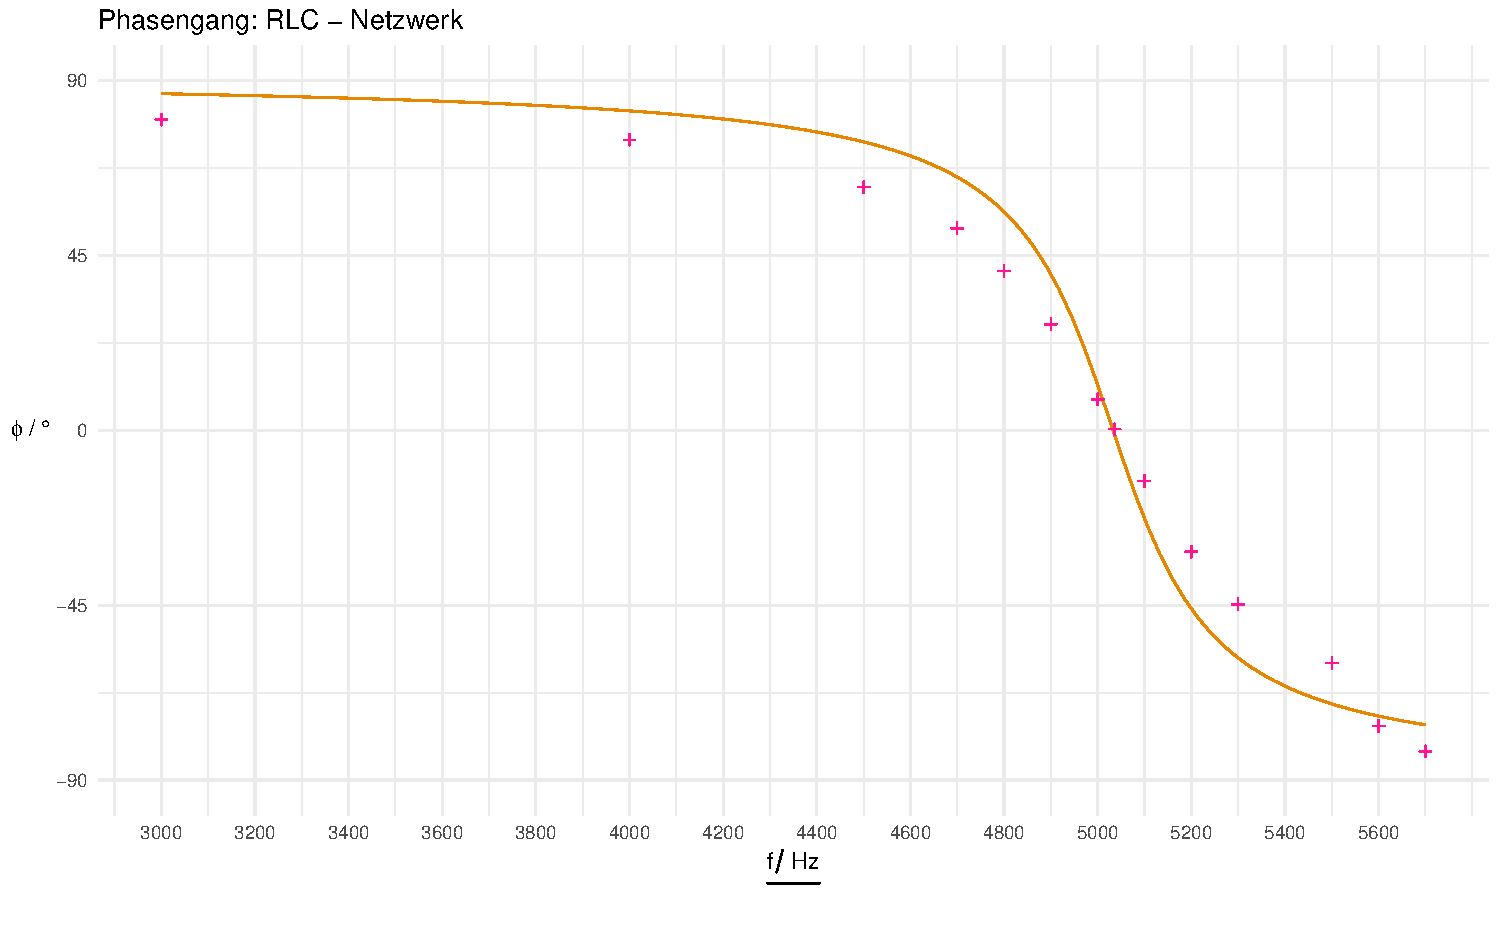
\includegraphics[scale=0.5]{./R/2_7/2_7_phase.pdf}
    \end{center}



\end{document}
